\documentclass[12pt]{paper}

\usepackage{Schwieg}
\usepackage[margin=1in]{geometry}
\usepackage{tikz}
\title{Price Theory I: Problem Set 1.2}
\author{Samuel Barker\and Timothy Schwieg\and Rafeh Qureshi\and Daniel Noriega\and Ana Vasilj}
\begin{document}
\maketitle

Given: there are two regions: north and south; the exterior temperature in the north ($T_N$) is always less than the exterior temperature in the south ($T_S$); people have preferences on one good $X$ and on the interior temperature of their house ($H$); people can raise $H$ by $K$ by spending $K*C(I)$ where $I$ is the amount of insulation and $C'(I)<0$; and finally that wages in a region depend negatively on the amount of people in that region.

Assumed: utility functions are the same for all individuals and are strictly quasi-concave; individuals are free to move between regions; and the ideal temperature is higher than the current external temperature in both north and south (i.e. everyone prefers higher temperatures for their houses relative to the exterior temperature).

\section{Part A}
Q: Assuming insulation in the north and south are fixed at the same level, how will wages, consumption of $X$, and $H$ differ?
\\

To answer this question, we will work our way back from an equilibrium condition.
\\

\textbf{Claim: $u(X_N,H_N)=u(X_S,H_S)$ in equilibrium.}

This follows from the fact that if $u_N>u_S$ then people would move north. Informally, this would result in $w_N$ falling and $w_S$ rising until $u_N=u_S$.
\\

\textbf{Claim: $X_N=X_S$ and $H_N=H_S$ in equilibrium.}

This claim follows from two facts: the utility functions are the same, and they face the same prices (i.e. $P_X$  and $C(I))$. Because they face the same prices, the slope of the budget line is the same and the $X$ and $H$ for which they are tangent would have to be the same. We know that in equilibrium the slope of the budget line is the same as the slope of the line tangent to the utility curve and, by strict quasi-concavity, this spot on the utility curve is unique. Thus there is a unique $X^*$ and $H^*$ such that $u^{'}_i(X^*,H^*)=\frac{C(I)}{P_X},~i\in  \{N,S\}$ (where the right hand side is the slope of the budget line).
\\

\textbf{Claim: $K_N>K_S$, $w_N>w_S$, and there are more people in the south than in the north.}

The first fact comes immediately from $H^*=H_N=H_S.$ Notice that $H_N=T_N+K_N=T_S+K_S=H_S$, and we know that $T_S>T_N \implies K_N>K_S$.

The second fact follows from the first. In equilibrium $w_i=P_XX_i+C(I)K_i,$ thus we can construct backwards what income looks like in each region relative to each other. Specifically, it follows that:
\begin{align*}
K_N&>K_S\\
K_NC(I)&>K_SC(I)\\
P_XX+K_NC(I)&>P_XX+K_SC(I)
\end{align*}
These are just the budget constraints for the north and south respectively. We know that in equilibrium, wage will be equal to total expenditure, and thus:
\begin{align*}
w_N=P_XX+K_NC(I)&>P_XX+K_SC(I)=w_S\\
\implies w_N&>w_S.
\end{align*}

It is given that wages are negatively related to the population of a region. Therefore, we can induce our third result: there are more people in the south than the north because $w_N>w_S$.

It is useful to visualize what is being said here. Refer to Fig. 1: 2-a.  Here you will see the utilities of north and south plotted on an axis of $X$ and $K$. $u_N$ has been shifted over to the right because for the same $X$ they must consume more $K$ than the southerners (to be precise, it must be the case that $K_N-K_S=T_S-T_N$) to achieve the same utility as those in the south. It is also apparent that since the slope of the tangent line is the same, they must have the same value of $X$. And lastly, there is an obvious need for a higher wage in the north, which implies that people have sorted themselves out to have a higher population in the south.

\section{Part B}
Q: What will happen to wages and house temperatures in both regions if there is an equal increase in insulation in both places?
\\

To model this, imagine that insulation has been added to houses and wages have not adjusted yet. Denote the state before the insulation increase as state $0$, and after as state $1$.

If wages have not adjusted yet, then: 
\begin{align*}
w_{N_1}-w_{N_0}=0&=w_{S_1}-w_{S_0}\\
w_{N_1}-w_{N_0}=&~w_{S_1}-w_{S_0}
\end{align*}
Because wages will equal expenditure, we also have:
\begin{align*}
P_XX_1+C(I_1)K_{N_1}-P_XX_0-C(I_0)K_{N_0}&=P_XX_1+C(I_1)K_{S_1}-P_XX_0-C(I_0)K_{S_0}
\end{align*}
Realize that because north and south face a budget constraint with the same slope again, there once again exists a unique $X^*_1$ such that the slope for $u$ at that point is equal to the budget line in both regions. This implies that $X_{N_1}=X_{S_1}$, which is why a general $X_1$ has been used. This also means that we can cancel out $P_XX_0$ and $P_XX_1$ from each side. We then get:
\begin{align*}
C(I_1)K_{N_1}-C(I_0)K_{N_0}&=C(I_1)K_{S_1}-C(I_0)K_{S_0}\\
C(I_1)(K_{N_1}-K_{S_1})&=C(I_0)(K_{N_0}-K_{S_0})
\end{align*}
Because $C'(I)<0$, and $I_1>I_0$, we have that $C(I_1)<C(I_0)$. This implies that:
\begin{align*}
K_{N_1}-K_{S_1}&>K_{N_0}-K_{S_0}
\end{align*}
The reason we know that the inequality goes this direction is because we have that $K_{N_0}>K_{S_0}$ (there is no nonsense with negatives being multiplied). The important result from this is the household temperature in the north and south is no longer equal after the insulation increase--this is the income effect. However, we established that consumption of $X$ in north and south is equal. Thus, if $H_{N_1}>H_{S_1}$, we would have that $u(X,H_{N_1})>u(X,H_{S_1}).$


A person can get more utility in the north right after the increase in insulation. Utility maximizing people would then move to the north, causing the wage in the north to fall, and the wage in the south to rise until the utilities equalize. When the utilities are equal, the binary relations from Part A still hold. Namely: $X$ is the same for north and south; $H$ will be the same for north and south; wages in the south are lower than in the north;  $K_N>K_S$; and the number of people in the south is greater than in the north. However, with an increase in $I$, the wage gap (and therefore population gap) between north and south will be smaller; both will spend more on $K$ and less on $X$ (substitution effect, and obvious from the budget line slope change (See Fig. 2: 2-b). Both the north and south utilities would have increased.

\section{Part C}
Q: If people can buy insulation at a constant price $P_I$, the how will the amount of insulation, consumption of $X$, household temperatures, and energy costs (i.e. $KC(I)$) differ across regions?
\\

Imagine that in part C we find ourselves with the people we left off in part B. We know that in part B, a decrease in $C(I)$ (or, equivalently, an increase in $I$) benefited the north more than the south. Let us suppose that for both it is beneficial to spend some of their wage on $I$ in order to achieve cheaper $K$ and that they both experiment by buying the same amount of $I$--call it $I_{experiment}$. In this case, the fall in money for buying $X$ and $K$ will fall in the north and south by the same amount: $I_{experiment}*P_I$ (note that $P_I$ is given and constant across regions). For this, we already know from part B that the north will benefit more than the south from this decision. Therefore, individuals will move from the south to the north causing the wage gap to close shrink. 

This process will continue until eventually the south will not find it beneficial to buy more $I$. But, at this point, the north will continue to buy more $I$--again, from B they benefit more, and thus when the south benefits not at all, the north will benefit some. Thus, the north will end up buying more $I$:
\[
I_N>I_S.
\]

This result immediately implies $C(I_N)<C(I_S)$. Thus, the absolute value of slope of the budget line for the north is less than the absolute value of the slope for the south. i.e.:
\[
\frac{C(I_N)}{P_X}<\frac{C(I_S)}{P_X}.
\]
This suggests to us that $X_S>X_N$ and $K_N>K_S$. And because we know that in equilibrium $u_N=u_S$, and $X_S>X_N$, then it must be the case that $H_N>H_S$, which is consistent.

We also still get that $w_N>w_S$. This is obvious from the fact that if $w_N=w_S$, then for any $X$, the people in the south could achieve a higher $H$ than the people in the north because of the fact that $T_S>T_N$. If this were true, then the utilities would not be equal, and people would move to the south causing the wages in the north to become greater than the wages in the south. And, if $w_N>w_S$, then:

\begin{align*}
P_XX_N+C(I_N)K_N&>P_XX_S+C(I_S)K_S\\
\text{and by } X_N&<X_S \text{ we get}\\
C(I_N)K_N&>C(I_S)K_S
\end{align*}
Thus, cost of energy in the north is greater than the cost of energy in the south.


Note that we could imagine this experiment in reverse--where both north and south benefit from selling off their $I$ to someone (though who this person is is a mystery). In this case, the south would benefit from selling off $I$ more than the north, and thus we would eventually reach the same results that we reached above.


To answer the question posed explicitly: people in the south will consume relatively more $X$, people in the north will have relatively higher interior temperatures, the cost of energy will be higher in the north (i.e. $K_NC(I_N)>K_SC(I_S)$) and northerns will face lower $C(I)$ because they will have more insulation.

For a visual aid, refer to Fig. 3: 2-c. It shows one possible case of allowing people to purchase $I$ (though all cases would have the same results as listed above, their graphs could pop up differently, for instance, the budget curves for north and south could intersect, etc.).

\begin{figure}
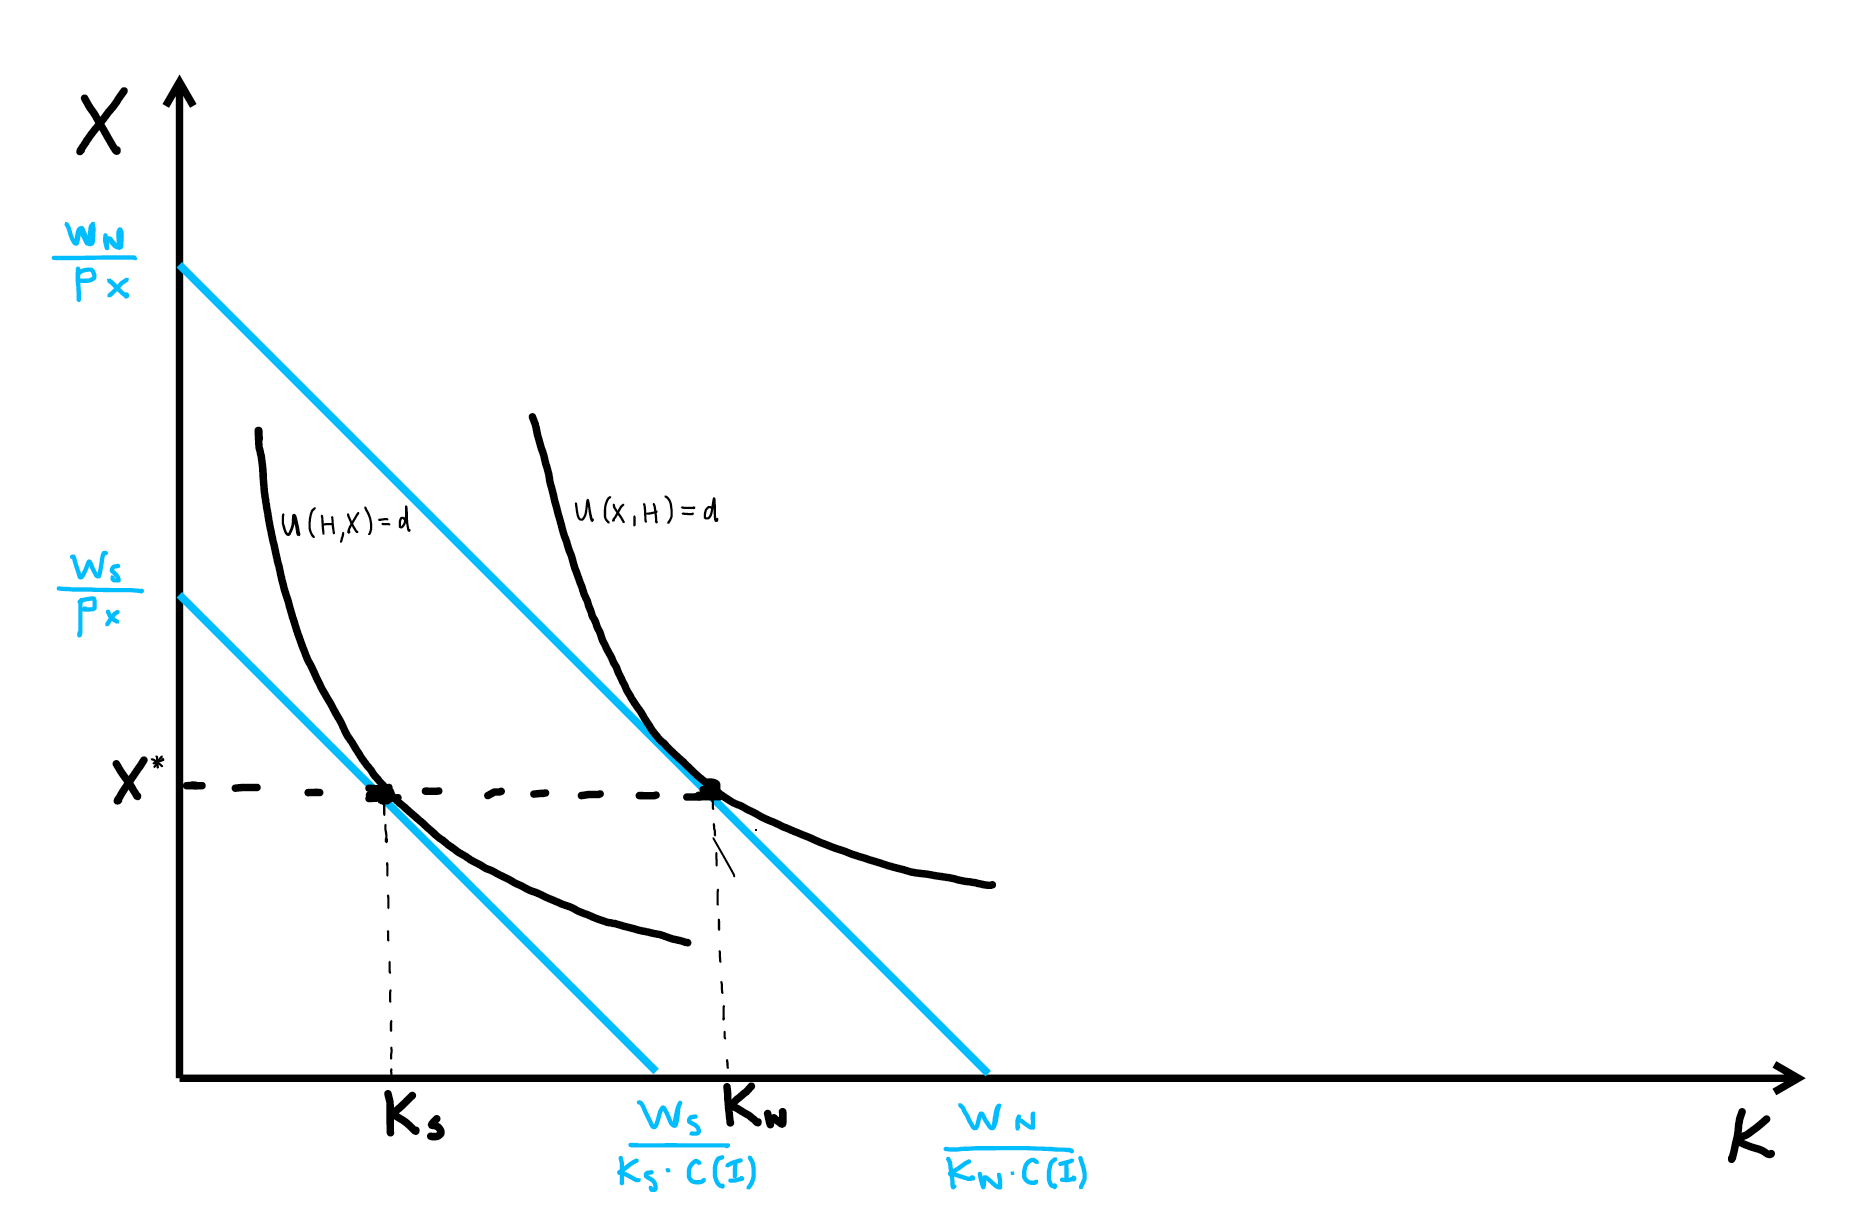
\includegraphics[width=\textwidth]{2-a}
\caption{2-a}
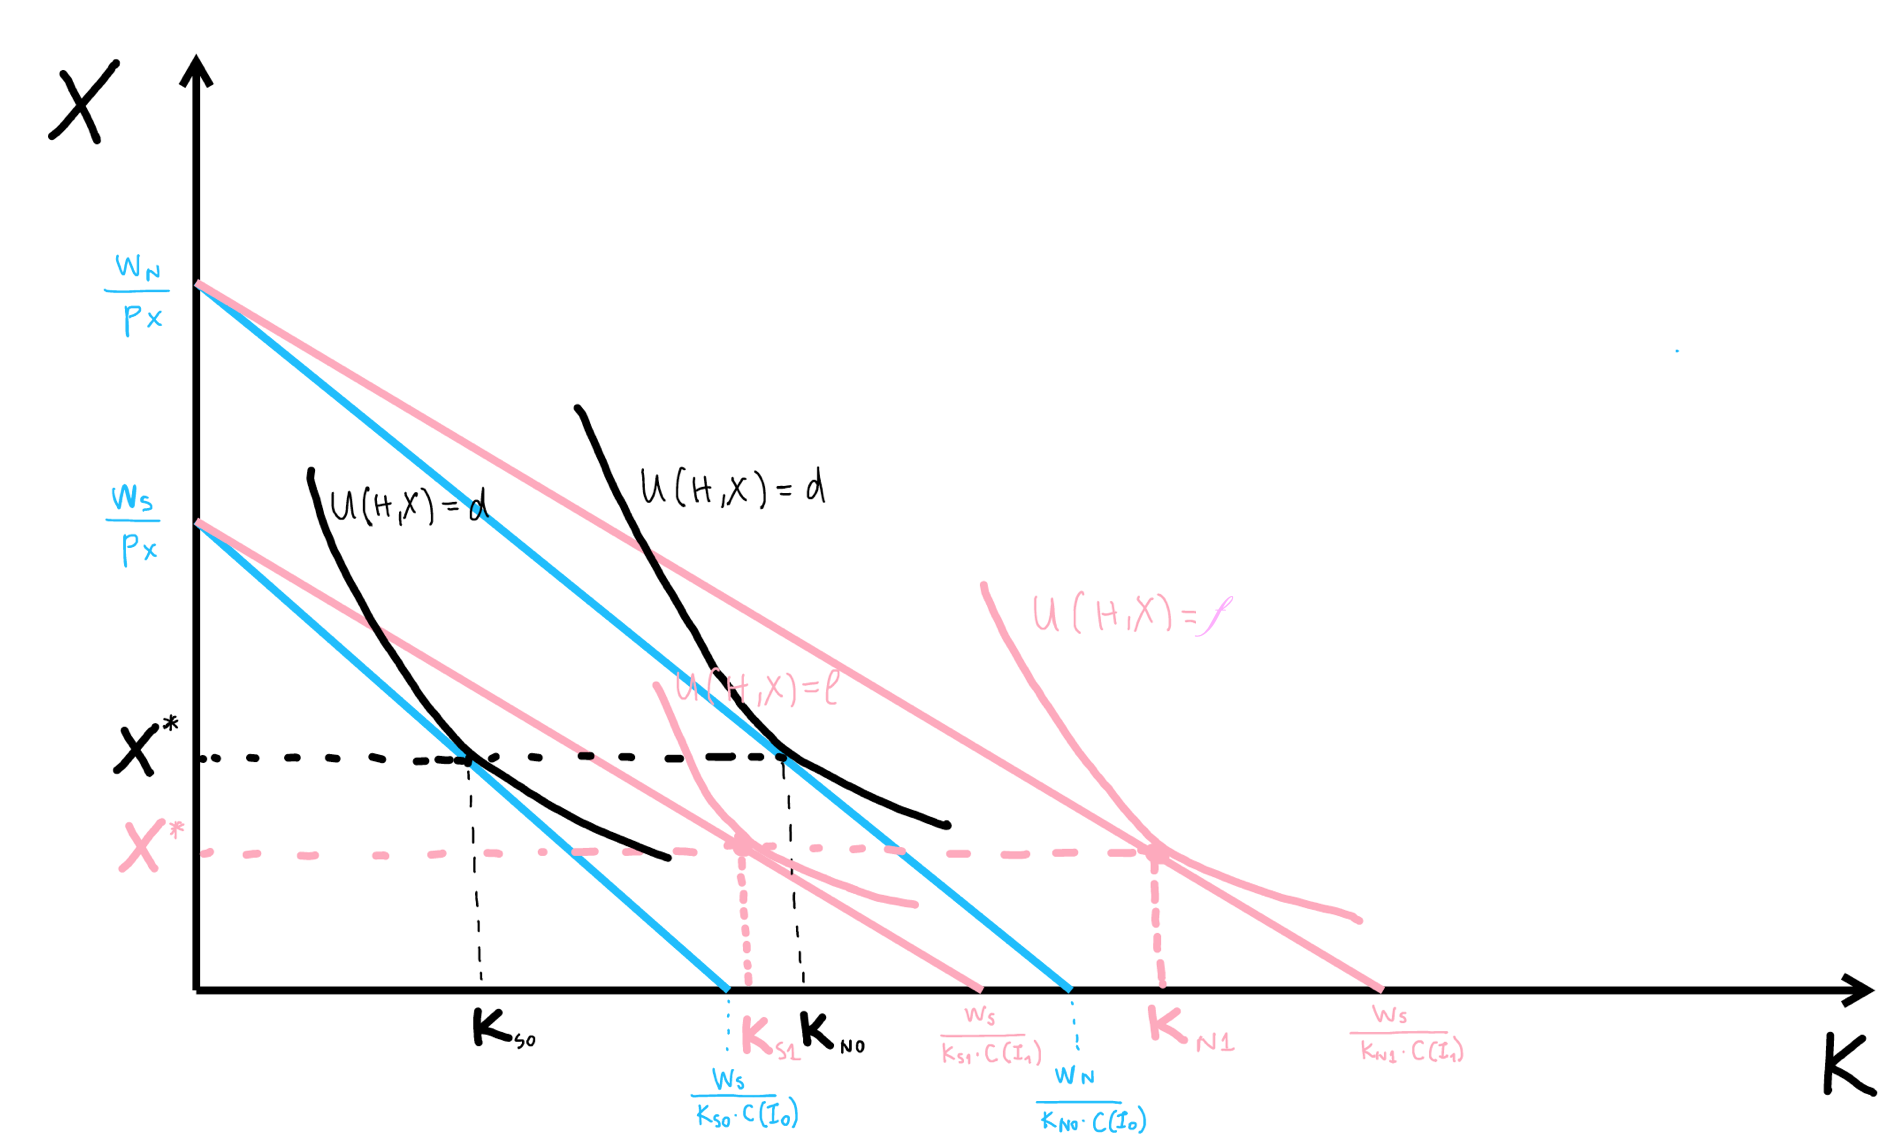
\includegraphics[width=\textwidth]{2-b}
\caption{2-b}
\end{figure}
\begin{figure}
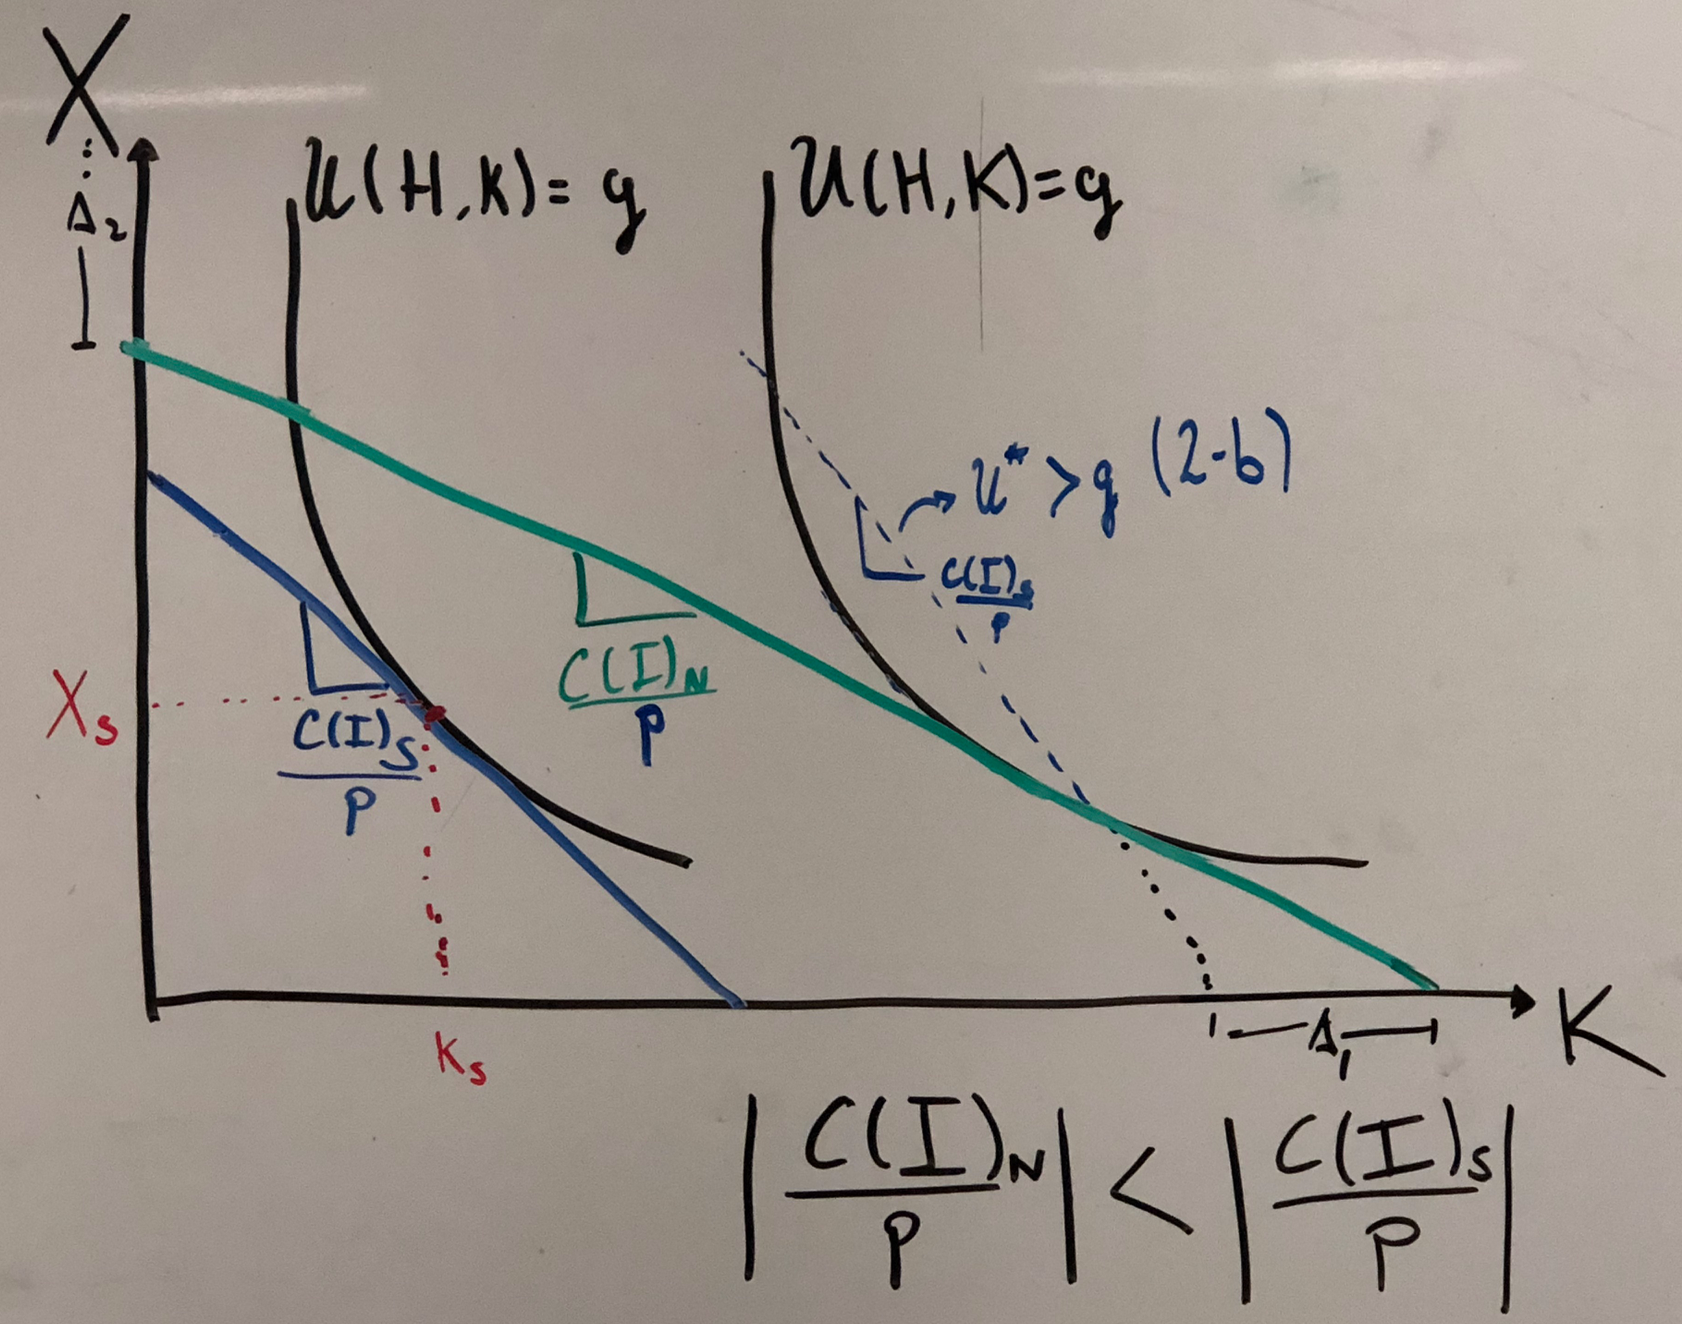
\includegraphics[width=\textwidth]{2-c}
\caption{2-c}

\end{figure}

\begin{align*}
\end{align*}





\end{document}